
\title{15-440: Lab 2}
\author{
        Spencer Barton (sebarton)\\
        Emma Binns (ebinns)
}
\date{September 11, 2014}

\documentclass[12pt]{article}

\usepackage{graphicx}
\usepackage[compact]{titlesec}
\usepackage[letterpaper, portrait, margin=1in]{geometry}
\usepackage{amsmath, amsfonts, amsthm, amssymb}

\setlength{\parindent}{0pt}
\setlength{\parskip}{\baselineskip}

\begin{document}
\maketitle

%------------------------------------------
\pagebreak
\section{Design}

Here is a UML diagram to illustrate our design:

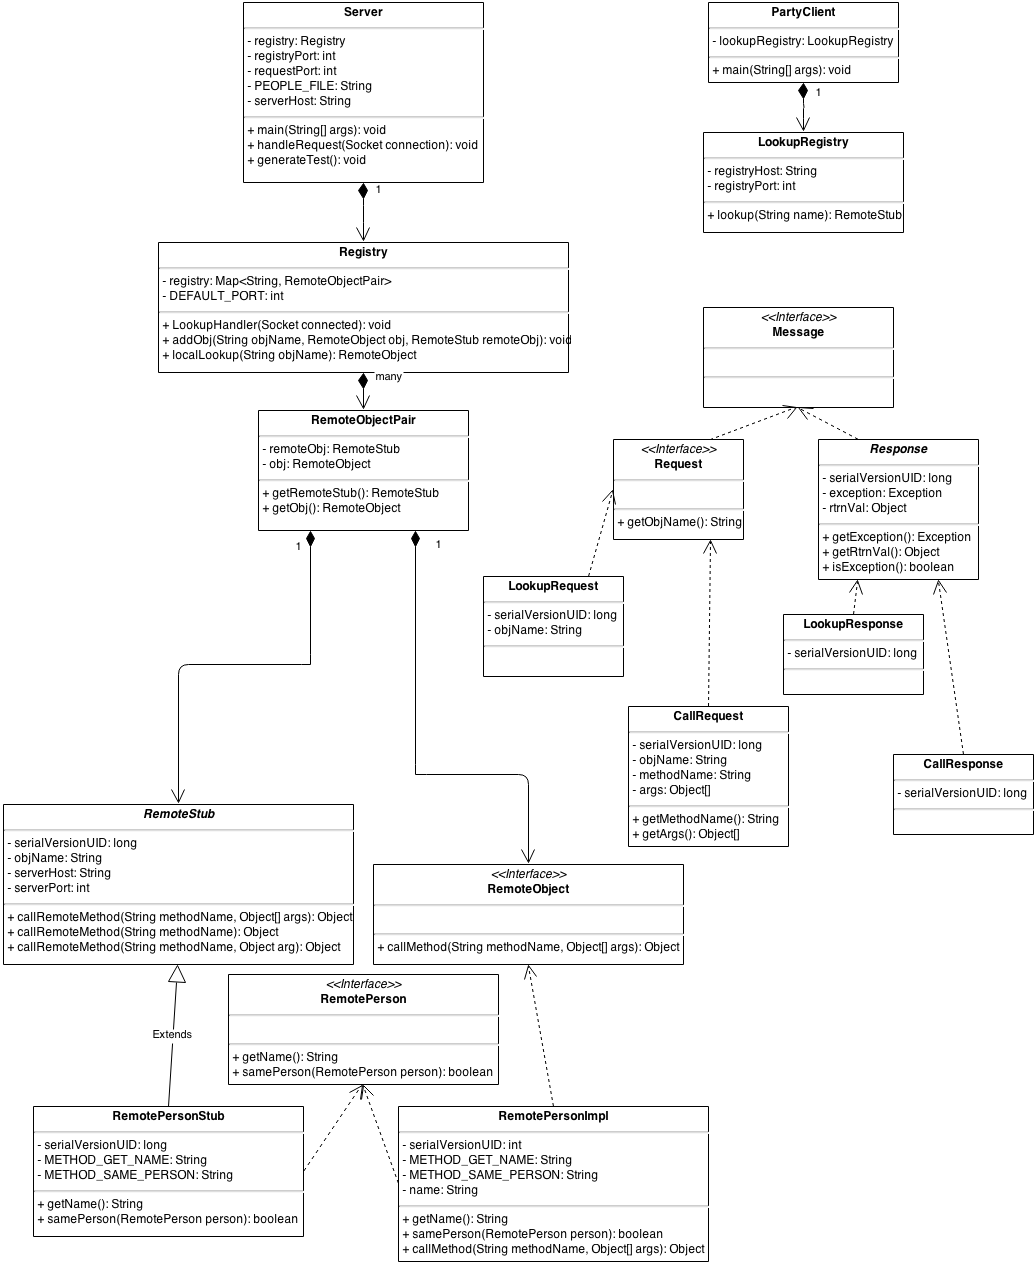
\includegraphics[scale=.44]{UMLsized.png} \\

We decided not to implement any server skeletons and instead to incorporate the functionality of a dispatcher into our server. We chose to do this because, as stated in the handout, the process to handle remote method calls is not dependent on the specific object the method is being called on. Therefore, it made more sense to us for our server to include the functionality of a dispatcher rather than having each stub require a corresponding skeleton.

\texttt{PartyClient} and \textttt{RemotePerson} are simply a demonstration client and remote object.

\subsection*{Registry Lookup}

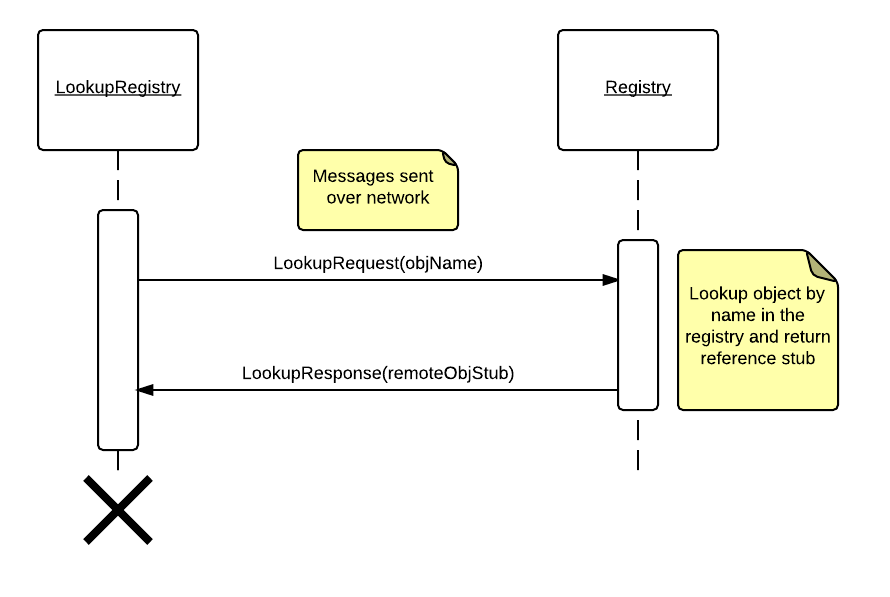
\includegraphics[scale=.4]{Lookup.png}

In order to lookup a remote object the client uses their \texttt{LookupRegistry} to lookup an object by name string. The \texttt{LookupRegistry} creates a \texttt{LookupRequest} with the object name. This is sent to the server which looks up the object by name in its registry. If the object exists, a \texttt{RemoteObjectStub} is returned through a \texttt{LookupResponse} else the \texttt{LookupResponse} comes back with an exception.

\subsection*{Remote Method Invocation}

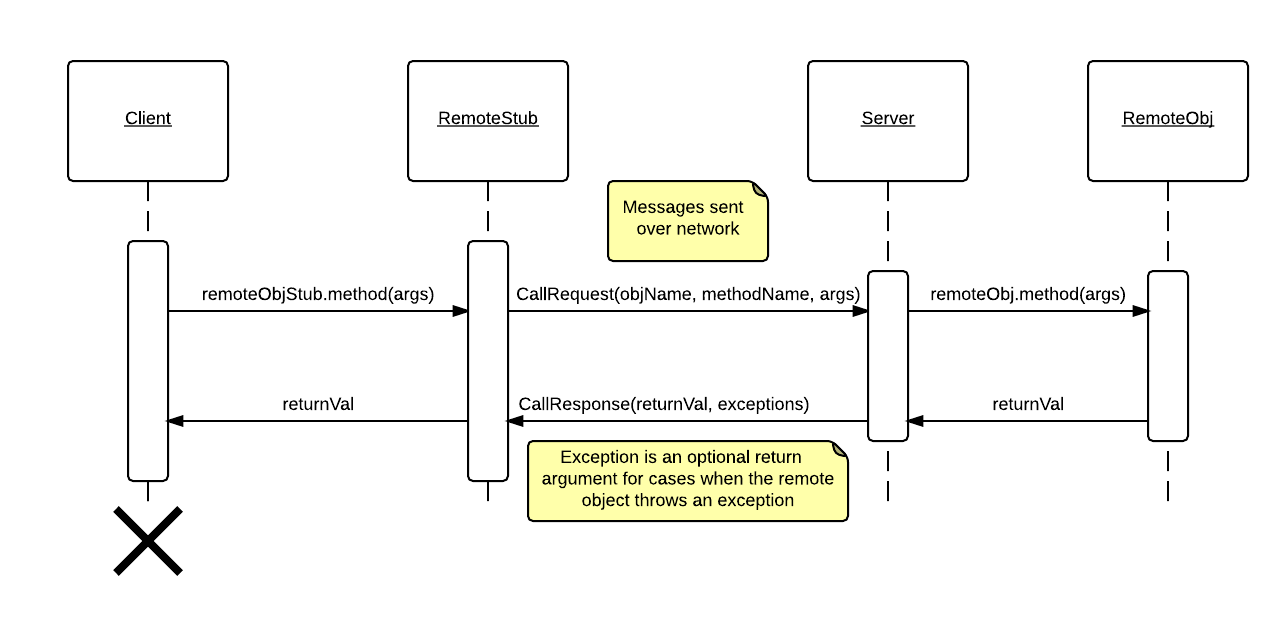
\includegraphics[scale=.3]{callMethod.png}

Remote object invocation begins with the client calling a method on a \texttt{RemoteObjectStub}. This call is then abstracted and a \texttt{CallRequest} message is generated with the object name, method name and arguments list. This message travels over the network to the server where the actual object lives. The relevant method is call and the return values is sent back to the client and returned from the original stub method invocation.

%------------------------------------------

\section{Implementation State}

We completed the basic requirements.

The extras that were not added include a skeleton, compiler and loading class files. We chose not to implement skeletons as we were able to add that the necessary methods within \texttt{RemoteObject}.

In order to add a compiler the design would not need to change. When performing a registry lookup a remote object stub is returned. Currently this remote object stub must be instantiated earlier by the server. With a compiler this would simply be replaced by a call to the compiler during an object lookup.

Finally support for loading class files would require a little more work since another server socket would need to be implemented on the host the .class files. Beyond that the remote object stub would handle a .class request and another type of message could be implemented to handle this communication.

%------------------------------------------

\section{Running the Project}

Here are the instructions to run our project on the Andrew machines using the provided example client/remote object code for testing: 

\begin{enumerate}
	\item{Navigate in a terminal to the directory containing our project, then navigate to the "src" folder within our project.}
	\item{Run the command: \verb|python SETUP.py| \\ (This command should print out commands to run the server and client.)}
	\item{From this "src" folder, run the server using the command: \verb|java server/Server| \\ (This command should print out: \verb|Server online at <hostname:port>|)}
	\item{In another terminal window (connected to a different server or the same one, whichever you prefer), navigate to the "src" folder as you did before. Then run the command: \verb|java client/PartyClient <hostname>| where \verb|<hostname>| is the hostname printed out when you ran the server above (this is the hostname corresponding to where you're running the server; ex: unix1.andrew.cmu.edu)}
\end{enumerate}

When you run the client, several lines should print out, both in the server window and the client window. These are the results of built in tests we've written that run automatically when you start the client. To check that our project works, we've provided thorough print statements of what is occurring at each step of the process. If our project functions correctly, this is what should print out:

\begin{align*}
	&\text{In the client window:} \\
	&\texttt{Creating local people} \\ \\
	&\texttt{Getting remote people} \\
	&\texttt{Sending lookup request from client to registry...} \\
	&\texttt{Lookup request result: <specific RemotePersonStub object>} \\
	&\texttt{Sending lookup request from client to registry...} \\
	&\texttt{Lookup request result: <specific RemotePersonStub>} \\
	&\texttt{Sending lookup request from client to registry...} \\
	&\texttt{Lookup request exception: java.lang.NullPointerException} \\
	&\texttt{Good - unable to find non-existant remote person} \\ \\
	&\texttt{These people are at the party:} \\
	&\texttt{Remote method call: calling getName on elain} \\
	&\texttt{Remote method call result: elain} \\
	&\texttt{Remote method call: calling getName on robert} \\
	&\texttt{Remote method call result: robert} \\
	&\texttt{sally ben jim robert elain robert} \\ \\
	&\texttt{Remote method call: calling getName on robert} \\
	&\texttt{Remote method call result: robert} \\
	&\texttt{Was Robert double counted (should be true)? true} \\
	&\texttt{Remote method call: calling samePerson on robert} \\
	&\texttt{Remote method call result: true} \\
	&\texttt{To check again, was Robert double counted (should be true)? true} \\
	&\texttt{Remote method call: calling samePerson on robert} \\
	&\texttt{Remote method call result: false} \\
	&\texttt{Are Elain and Robert the same person (should be false)? false} \\ \\
	&\texttt{Remote method call: calling samePerson on robert} \\
	&\texttt{Remote method call exception: java.lang.NullPointerException} \\
	&\texttt{Good we got an exception null}
\end{align*}
\begin{align*}
	&\text{In the server window:} \\
	&\texttt{Server received registry lookup request} \\
	&\texttt{Registry is performing lookup.} \\
	&\texttt{Registry lookup: elain} \\
	&\texttt{Server received registry lookup request} \\
	&\texttt{Registry is performing lookup.} \\
	&\texttt{Registry lookup: robert} \\
	&\texttt{Server received registry lookup request} \\
	&\texttt{Registry is performing lookup.} \\
	&\texttt{Registry lookup exception: java.lang.NullPointerException} \\
	&\texttt{Server received method call request} \\
	&\texttt{Remote method call request: elain.getName(null)} \\
	&\texttt{Server received method call request} \\
	&\texttt{Remote method call request: robert.getName(null)} \\
	&\texttt{Server received method call request} \\
	&\texttt{Remote method call request: robert.getName(null)} \\
	&\texttt{Server received method call request} \\
	&\texttt{Remote method call request: robert.samePerson(<specific Object>)} \\
	&\texttt{Server received method call request} \\
	&\texttt{Remote method call request: robert.samePerson(<specific Object>)} \\
	&\texttt{Remote method call: calling getName on elain} \\
	&\texttt{Server received method call request} \\
	&\texttt{Remote method call request: elain.getName(null)} \\
	&\texttt{Remote method call result: elain} \\
	&\texttt{Server received method call request} \\
	&\texttt{Remote method call request: robert.samePerson(<specific Object>)}
\end{align*}

%------------------------------------------

\section{Dependencies}

There are no dependencies.

%------------------------------------------

\section{Testing}

Our test in built into \texttt{PartyClient}. It automatically runs when \texttt{PartyClient} is run. The test runs each of the methods in the \texttt{Person} object for both a remote and local implementation. \texttt{Person.samePerson} is run using both remote and local objects as arguments to check that the server-side remote object implementation can handle either object type as an argument.

\end{document}
